\section{WebPerson Dataset}

\subsection{Person-Centric Image Filtering}
In this study, we utilize the COYO700M dataset~\cite{kakaobrain2022coyo-700m}, a large-scale dataset that contains 747M image-text pairs collected from CommonCrawl, as our web-crawled images source. To filter high-quality person-centric images, we initially deploy the YOLOv11 model \cite{yolo11_ultralytics} to detect humans and extract bounding box coordinates. The specific workflow is illustrated in Fig.~\ref{fig:pipeline}, where images are retained based on the following criteria: \textit{(i)} shorter dimension exceeds 90 pixels, \textit{(ii)} aspect ratio between 1:2 and 1:4, and \textit{(iii)} human detection confidence above 85\%. Subsequently, YOLOv11-Pose \cite{yolo11_ultralytics} verifies pose integrity by requiring: \textit{(i)} visibility of at least eight keypoints, \textit{(ii)} presence of at least one hip keypoints and two head keypoints. This process yields 5 million high-quality human-centric images filtered from the COYO700M dataset.


\begin{figure}[t]
\centerline{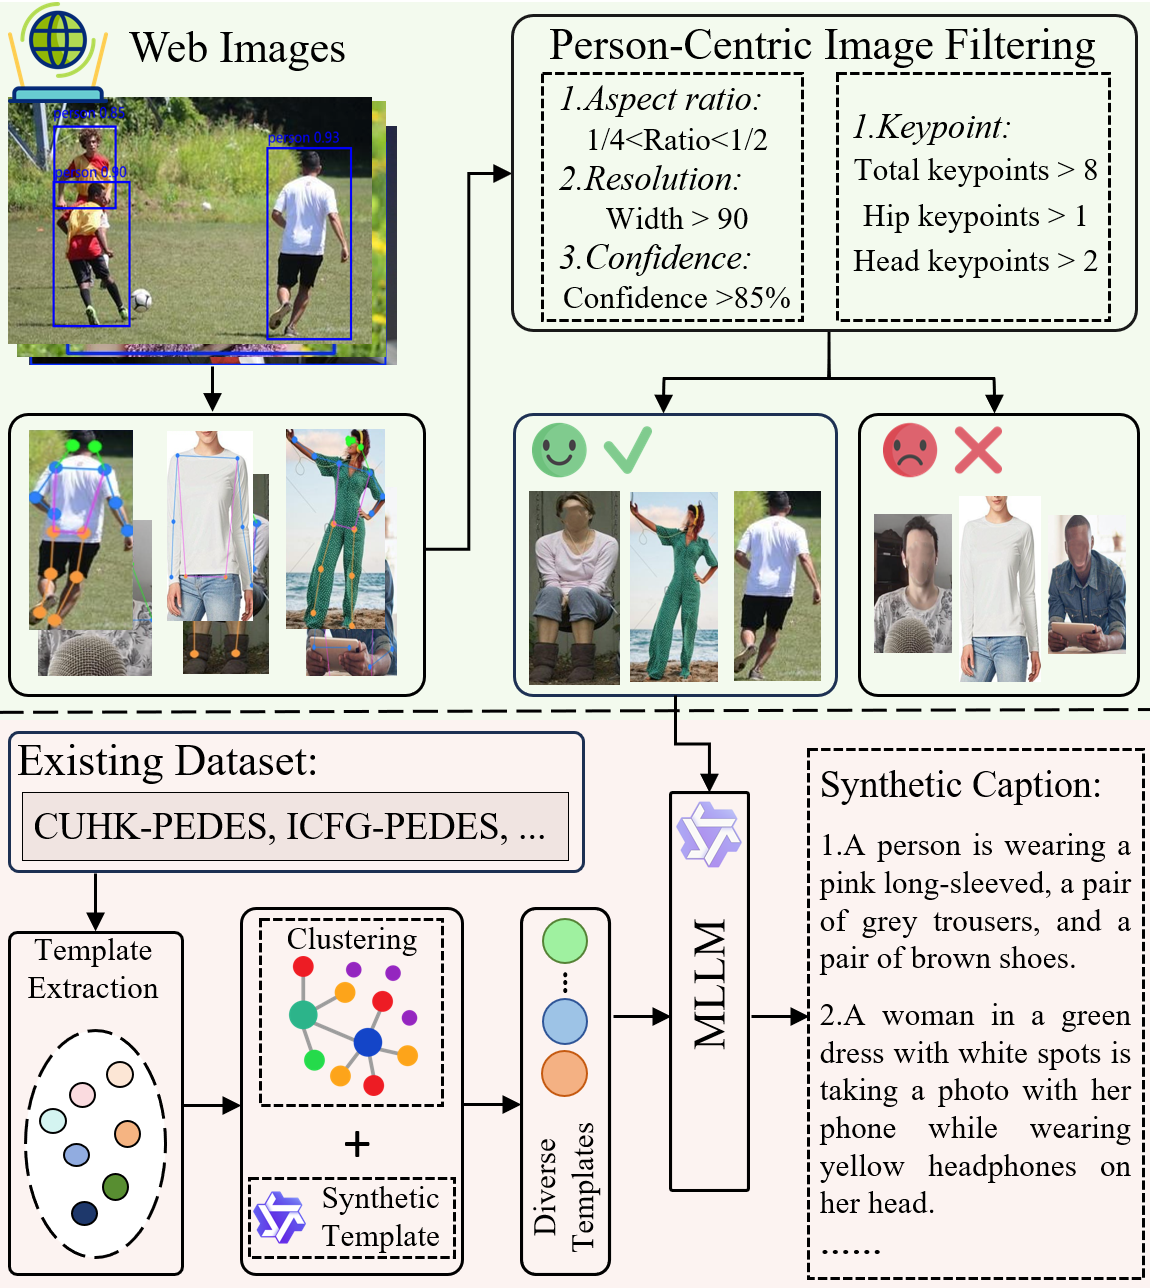
\includegraphics[width=\linewidth]{Figure/fig2_end.png}}
  \vspace{-2mm}
  \caption{The details of person-centric image filtering and synthetic caption generation pipeline for constructing our WebPerson dataset.}
  \label{fig:pipeline}
  \vspace{-5mm}
\end{figure}


\subsection{Synthetic Caption Generation}

Following the selection of 5 million high-quality human-centric images, we develop a synthetic caption generation pipeline to create diverse and precise textual descriptions. Our approach transforms existing captions from CUHK-PEDES~\cite{li2017person}, ICFG-PEDES~\cite{ding2021semantically}, and RSTPReid \cite{zhu2021dssl} into structured templates using Qwen2.5-72B-Instruct \cite{yang2024qwen2}. The model systematically replaces fine-grained attributes (\textit{e.g.}, black jacket, ponytail) with standardized placeholders (\textit{e.g.}, \texttt{[colored top]}, \texttt{[hairstyle]}). %The prompt for this transformation is detailed in the Appendix.

\begin{figure*}[t]
    \centering
    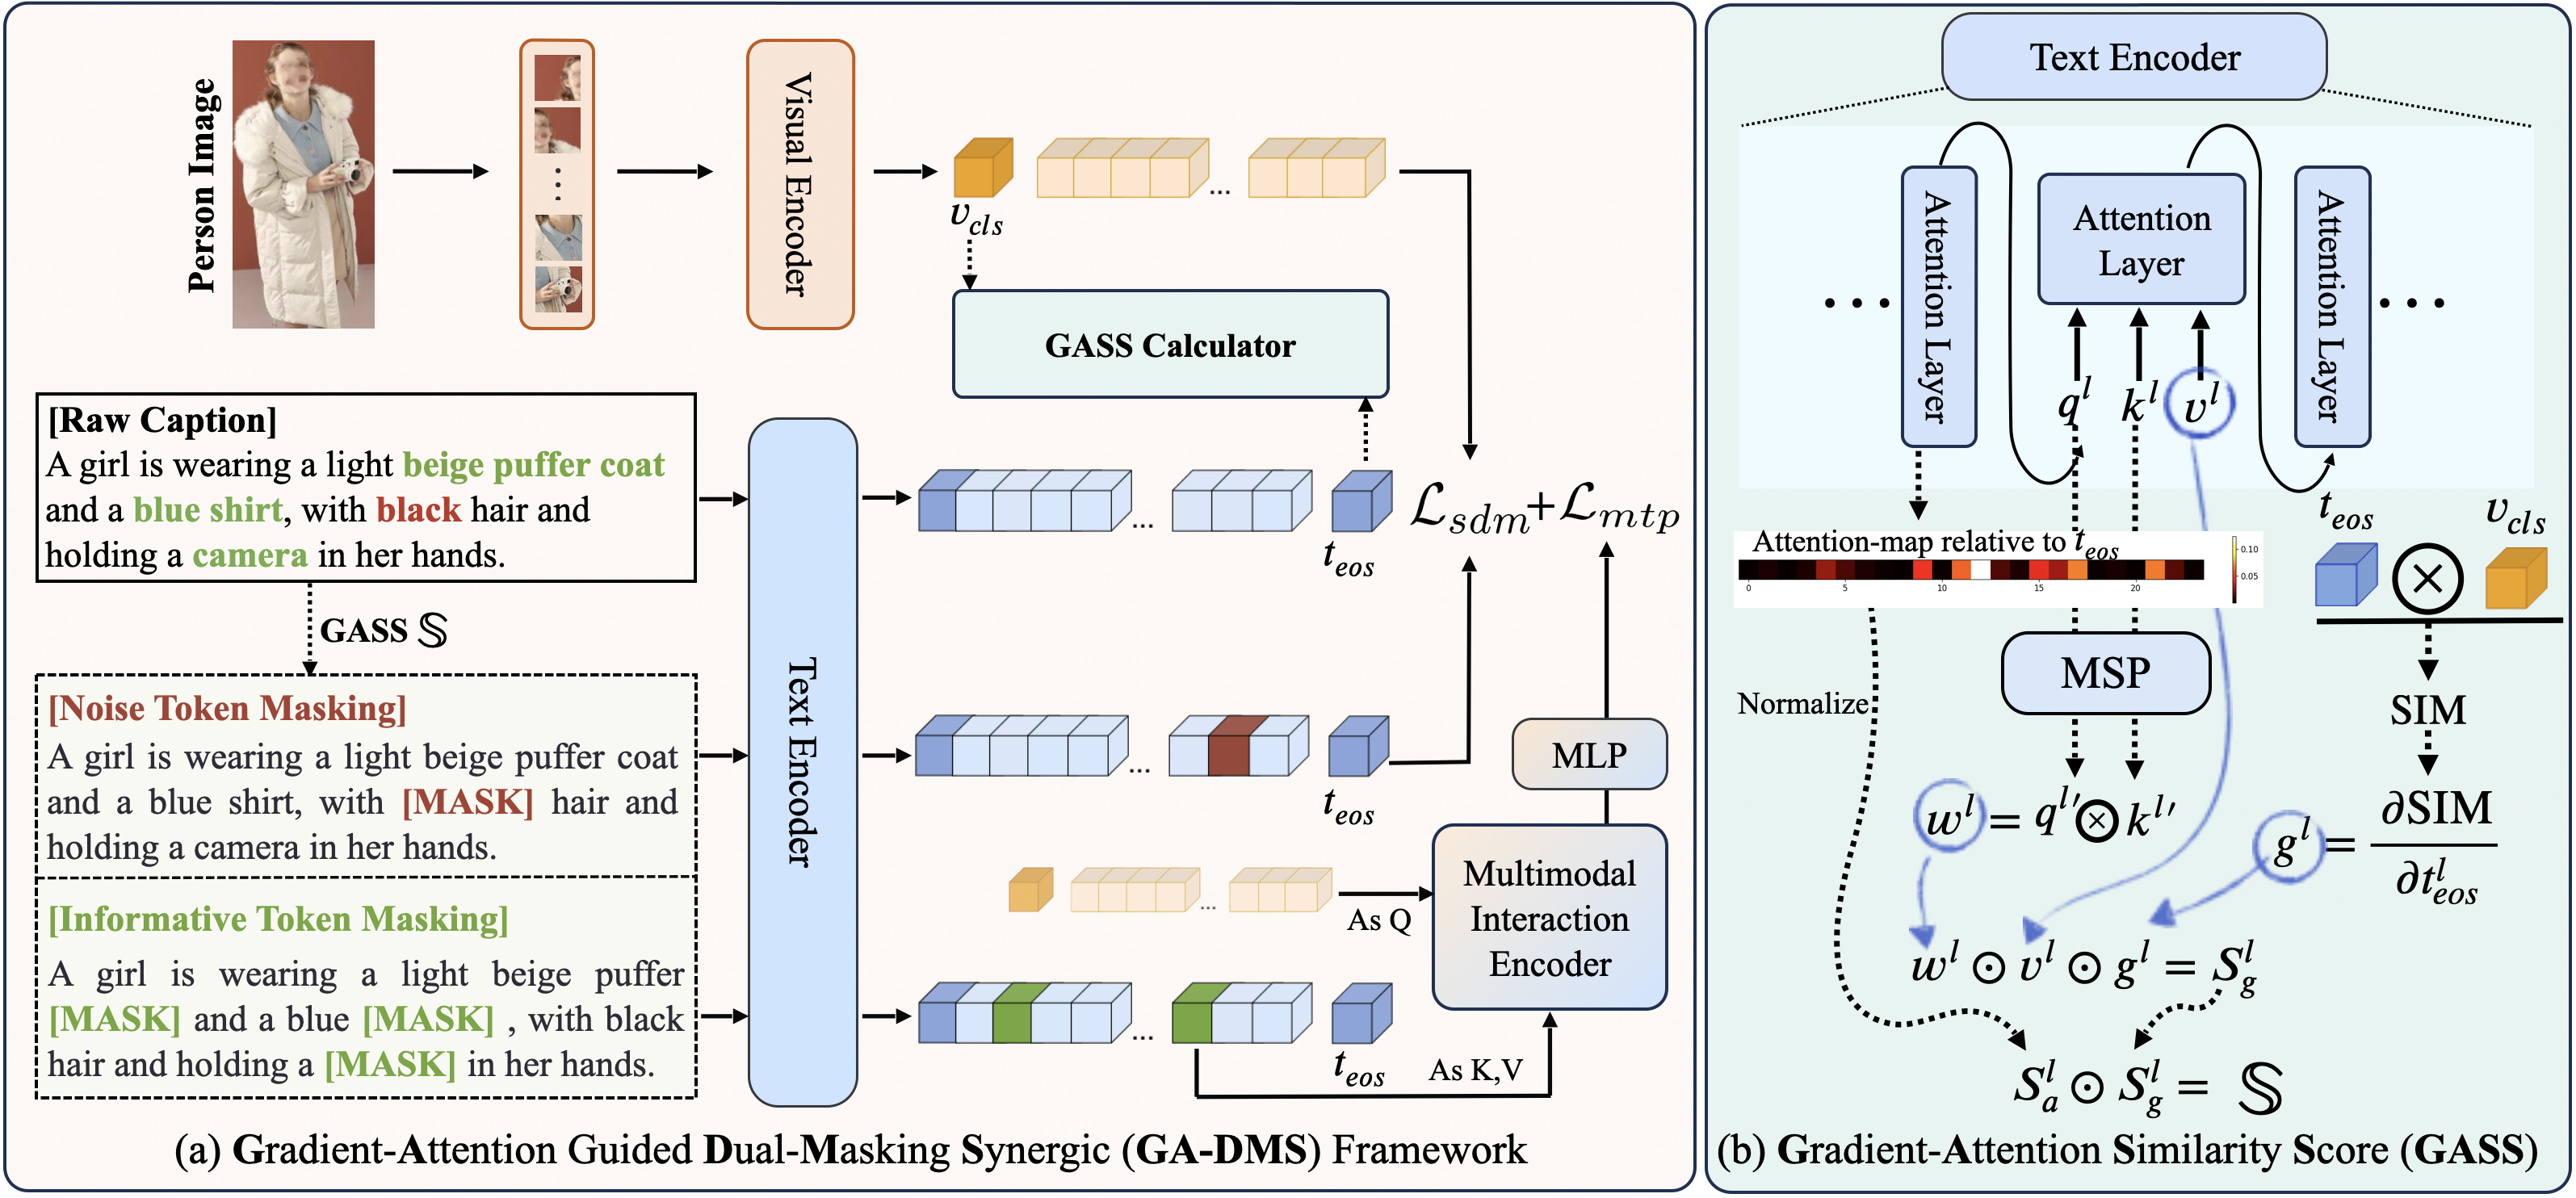
\includegraphics[width=\linewidth]{Figure/figure.png}
    \vspace{-7mm}
    \caption{Overview of our proposed method. (a) The architecture of our proposed Gradient-Attention Guided Dual-Masking Synergic~(GA-DMS) framework. (b) The details of the Gradient-Attention Similarity Score~(GASS).}
    \label{fig:method}
    \vspace{-5mm}
\end{figure*}

To reduce redundancy and cluster semantically similar templates, inspired by the previous works~\cite{clipcid,realsyn}, we employ the OPENCLIP ViT-bigG/14~\cite{Radford2021LearningTV} to extract text embeddings of the template texts, then we utilize the standard $k$-means algorithm to partition all the templates embeddings into $k$ distinct clusters based on the nearest neighbor criterion. Within each cluster, we select the most representative template (highest cosine similarity to the centroid) along with five randomly sampled templates. To further enhance template diversity, we employ Qwen2.5-72B-Instruct \cite{yang2024qwen2} to synthesize new templates from this refined set. All generated templates undergo rigorous review to eliminate biases and stereotypes, yielding a curated collection of one thousand high-quality templates. To generate diverse, high-quality captions, we leverage the in-context learning capabilities of MLLMs~\cite{li2025taco,unime}. Specifically, we randomly assign a template to each image and use Qwen2.5-VL-7B-Instruct and Qwen2.5-VL-32B-Instruct \cite{bai2025qwen2} to produce captions that follow the given template. We adopt vLLM~\cite{kwon2023efficient} to accelerate large-scale inference. The details of the prompt are provided in the Appendix ~\ref{Appendix prompt}.